

\section{GRU vs. Transformer}
It is important here to compare the GRU chatbot with the larger Transformer based chatbot. Using our subjective qualifications we see that the GRU model answers with more variety than the transformer model. The important observation is that the hyper-parameter set for the Transformer model can be expanded and enlarged as needed before training. The GRU model cannot be trained successfully with an arbitrarily large hyper-parameter set. We can train a larger Transformer and obtain the benefit associated with this, namely better responses.

A single further observation is that the GRU model responds very quickly, while a transformer model may take more time relatively. This is not a problem for general applications, but for our purposes we cannot ignore the time spent by the transformer model when it is installed on a small computer like a Raspberry Pi. 

The respective value of each of the models changes slightly when you consider what platform they will be implemented on. The GRU responds more quickly and so it retains some worth.


\section{Turing Test}

The Turing Test concerns itself with the question of weather a computer is intelligent. Turing says that intelligence is too hard to describe, and that if the computer can convince you that it is intelligent then it is.

Weather this is right is beyond the scope of this paper. The people who trained the Generative Pre-training Transformer 2 were apprehensive about their model's ability to generate human speech. They felt the model worked too well. At first when they finished their model they decided not to release the largest version to the public for several months (Radford et al) \cite{radford2019language}. Ultimately they did release their large model.

The creators of the model used it differently than our chatbot implementation. They generated paragraphs of text, and it was determined at first that the ability of the model to impersonate a human was too great. It was felt that the model could be used to spam facebook and other social networking sites with content that was very convincing. If the model could be used to convince people to act badly, then it should not be released. Humans are susceptible to the sentiments of those they see as their peers. If the model was, for better or worse, passing the Turing test, then it should not fall into the wrong hands. This was the concern of the coders at the time.

Ultimately the large model was released, either because the developers decided the model was not as good as originally estimated, or because they didn't care. 

\section{Winograd Schema}

Winograd schemas are named after Terry Winograd. The idea is that there is a sentence presented that has two meanings. A computer finds these sentences challenging to understand, and that makes them interesting for the development of Artificial Intelligence.

An example follows.

\begin{center}
	\textbf{He didn't put the trophy in the suitcase because it was too [big/small]}
\end{center}

We can choose which bracketed term to use, and we must choose only one bracketed term. If we choose `big' then we are referring to the trophy. If we choose `small' then we are referring to the suitcase. Human beings can easily see the pronoun `it' refers to either the suitcase or the trophy. Computers have trouble with these determinations.

The Transformer, and the Scaled Dot-product Attention that it uses, lends itself to discussion of Winograd schema. Remember that the Attention scheme compares tokens to other tokens in the same sentence. 

In the chat bot example, we are less interested in the Winograd example because it doesn't come up often. However, in the case of the Generative Pre-training Transformer 2, and it's exhaustive training, it is interesting to consider the Winograd style example sentences.

There is a Winograd Schema Challenge and something of a formula for constructing your own Winograd schema (Wikapedia contributors). \cite{wiki:xxx}

\section{Word Usage}

We make a general assumption that our transformer model uses only a small subset of words that it has available to it. In the example below 2000 input lines were tested from the training set and only a small percentage of the vocabulary words are used by the models in the output. These sentences came from the movie dialog corpus. Some percentage of words are used repeatedly.

\begin{figure}[H]
	\begin{center}
		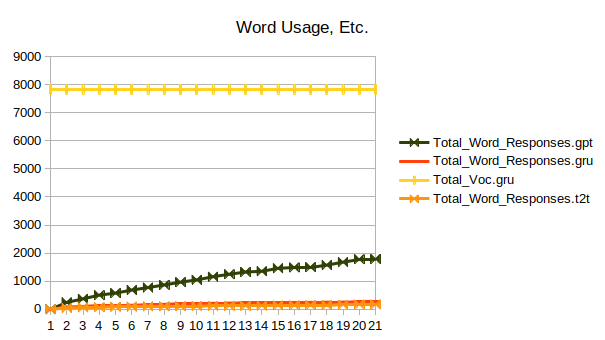
\includegraphics[scale=0.75]{Figure_5}
		
		
	\end{center}
	\caption[Word Usage]{Word Usage - Including Vocabulary Total}
	
	
\end{figure}

The yellow line at the top of the graph is the total words in the GRU vocabulary. The total words in the GPT2 vocabulary is not represented on the graph. Total responses in words are shown with the three remaining lines. The GPT2 responses are higher, and the GRU and Transformer responses look like horizontal lines at the bottom of the graph.

If we remove the Vocabulary Total and the GPT2 responses from the diagram the GRU output and the Transformer output take the shape of a curve with a limit somewhere below 300 words. The Transformer model has a vocabulary size of 8170 tokens. The GRU model is close to that at 7826 tokens. Both models use the same training corpus. The difference between the tokens available and the tokens used is large.


\begin{figure}[H]
	\begin{center}
		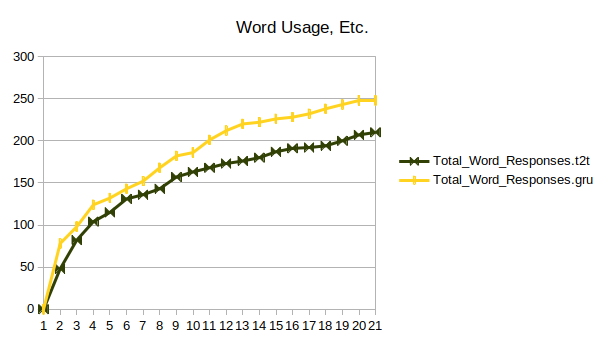
\includegraphics[scale=0.75]{Figure_6}
		
		
	\end{center}
	\caption[Simple Word Usage]{Simple Word Usage - No Vocabulary Total}
	
	
\end{figure}

We might conclude from these comparisons that the GRU model operates more robustly than the Transformer model. This may be the case, or the transformer model may be over trained or over fitted. It also might be that the hyper parameter set is poorly adjusted. We suspect the learning rate, for example, may be too high.

\section{Sentence Usage}

If we were interested in transfer learning and we wanted to train a model as a classifier, we might be interested in how many fully formed responses the given model uses. Additionally we might be interested in when or how many of these responses were used repeatedly.

The GPT2 model is very large and very versatile, but the Transformer model and the GRU model are smaller. For these two smaller models it would be good to tell how many repeated sentences occurred as output in some number of inputs. As above we use 2000 inputs from the training set of the movie dialog corpus.

We have a rough number for those two models. They use about 125 sentences repeatedly. As for total sentences used the Transformer uses fewer in total. The GRU is increasing still at 350 sentences at the end of our study. We assume that at some point the number of total GRU sentences that that model can produce reaches some kind of limit.

\begin{figure}[H]
	\begin{center}
		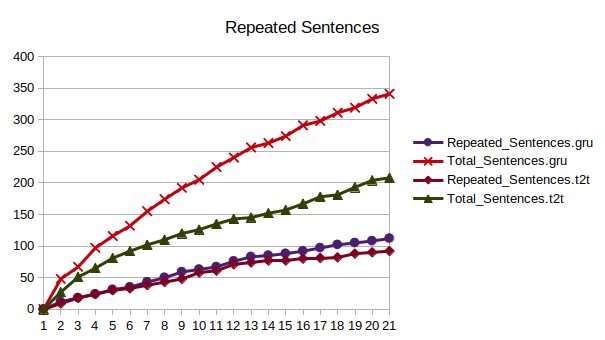
\includegraphics[scale=0.75]{Figure_8}
		
		
	\end{center}
	\caption[Simple Sentence Usage]{Simple Sentence Usage}
	
	
\end{figure}

\iffalse
In a transformer classifier we might be tempted to choose 125 sentences for the maximum number of classifications. If we were going to try to create a neural network model that was trained for a specific Q/A task using a transformer this might be important. We could use 125 as our maximum number of outputs. This is a relatively large number. Transformer classifier networks often have just a few classes.
\fi

The interesting thing is that the Transformer and the GRU models both have similar `Repeated Sentence' graphs. They are totally different models and have totally different sizes. They are not similar in many ways but in this metric. They share the same corpus, so they may be learning the same task.


\section{Transformer Chatbot Learning}

For the chatbot task we want to know what the Transformer is doing during training and later during inference. Here we are concerned with the Transformer model trained on the movie dialog corpus and not the GPT2 model. The Transformer model in question has 6 layers and a hidden size of 512 units.

It seems the model learns a set of multi-purpose English answers in a form close to a list. Then it spends time as a classifier. Each input sentence is compared to the set of answers. A question is associated with a given answer from the set when possible. There would be fewer answers than there are questions. It is as if there were a list somewhere that contained many of the answers that the model would use. For a given model this list can only be so long.

It is interesting to point out that probably at the start the multi-purpose answers are constructed at the same time that the classification task is taking place. 

We feel that this list making is a function of the model trying to optimize the answers that it gives, and can give, given a certain size memory capacity. The model has a certain capacity and it starts to develop lists of usable answers in order to use that capacity best.

We don't feel that the output of the Transformer, for example, shows intelligence. The actual utterances of the model are pretty plain. The internal building of lists, though, shows a process that is found in some intelligent activity.

For the very large pre-trained model, like the GPT2, this may not be true. These models may be more dynamic. In addition we have not done tests with translation tasks. For translation the same model may be able to remember longer lists, or in place of a list of complete responses keep a list of phrases or partial responses that could be combined to create translated output.
